\documentclass[a4paper,10pt,fleqn]{scrartcl}
\usepackage[utf8]{inputenc}
\usepackage[T1]{fontenc}
\usepackage{amsmath}
\usepackage{graphicx}

\date{}
\title{Algorithm development draft on angular-dependent backprojection}

\begin{document}
\maketitle
\paragraph{Point coordinate calculation}
\textbf{Note: All coordinares are relative to M}
\begin{align*}
E &= (r * cos(\alpha) | r * sin(\alpha)) \\
\delta &= 90^\circ - \alpha \\
G &= (x_E + r_e * \sin(\delta) | y_E + r_e * \cos(\delta)) \\
  &= (r * \cos(\alpha) + r_e * \sin(\delta) | r * \sin(\alpha) + r_e * cos(\delta))\\
  &= (r * \cos(\alpha) + r_e * \sin(90^\circ - \alpha) | r * \sin(\alpha) + r_e * cos(90^\circ - \alpha))\\
  &= (r * \cos(\alpha) + r_e * \cos(\alpha) | r * \sin(\alpha) + r_e * \sin(\alpha))\\
  &= ([r + r_e] * \cos(\alpha) | [r + r_e] * \sin(\alpha))\\
\overline{D\,S_D} &= (y_E - y_D) * \tan(90^\circ-\alpha) - (x_G - x_D) \\
\overline{A\,S_A} &= (y_E - y_A) * \tan(90^\circ-\alpha) - (x_G - x_A) \\
2 * A_E &= \overline{D\,S_D} + \overline{A\,S_A} \\ %Effect Amount
  &= (y_E - y_D) * \tan(90^\circ-\alpha) - (x_G - x_D) +\\&\qquad(y_E - y_A) * \tan(90^\circ-\alpha) - (x_G - x_A)\\
  &= (y_E - y_D) * \tan(90^\circ-\alpha) +\\&\qquad(y_E - y_A) * \tan(90^\circ-\alpha) - 2 * (x_G - x_A) \\
  &= [(y_E - y_D) + (y_E - y_A)] * \tan(90^\circ-\alpha) - 2 * (x_G - x_A)\\
\end{align*}
\textbf{Complexity:}
\begin{equation}
\mathcal{O}(x^3)
\end{equation}
\newpage
\paragraph{Case 1:}
\begin{figure}[h]
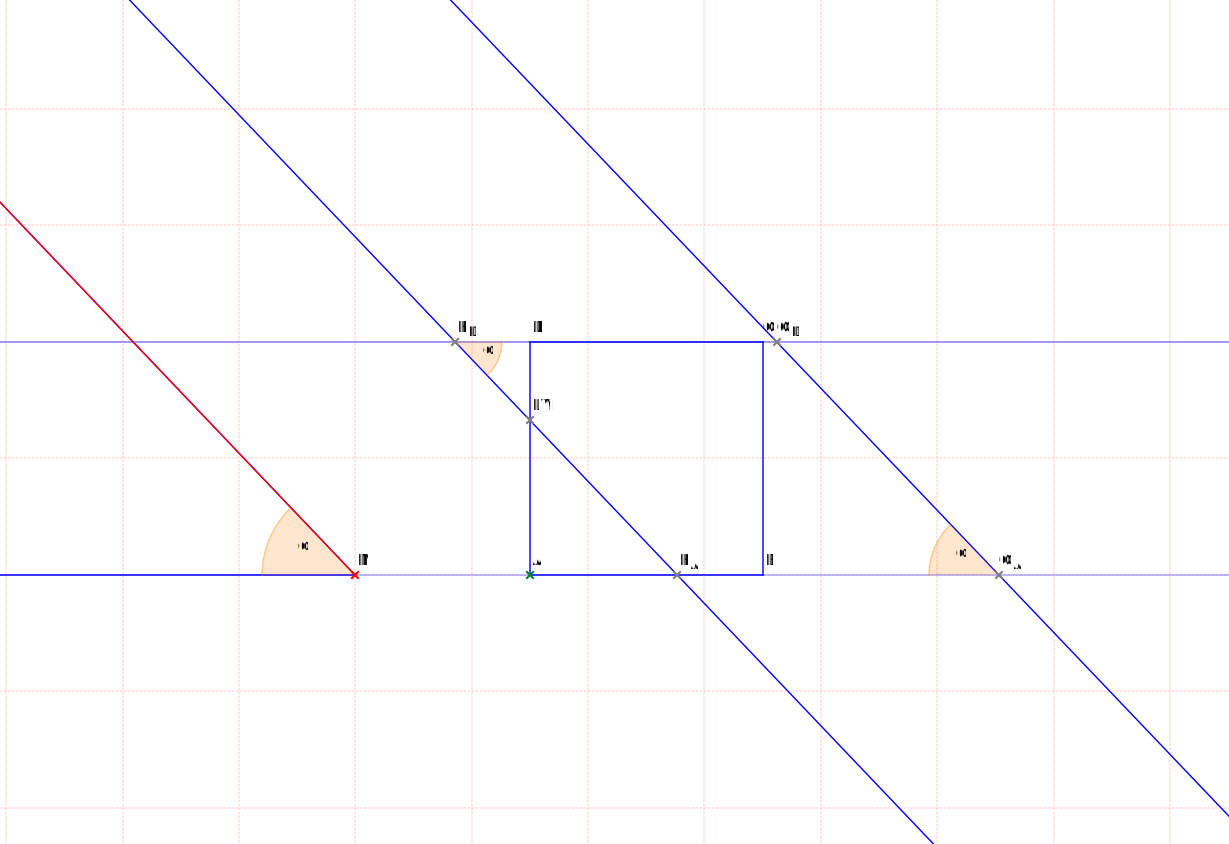
\includegraphics[width=0.8\textwidth]{case1}
\end{figure}
\paragraph{Case 2:}
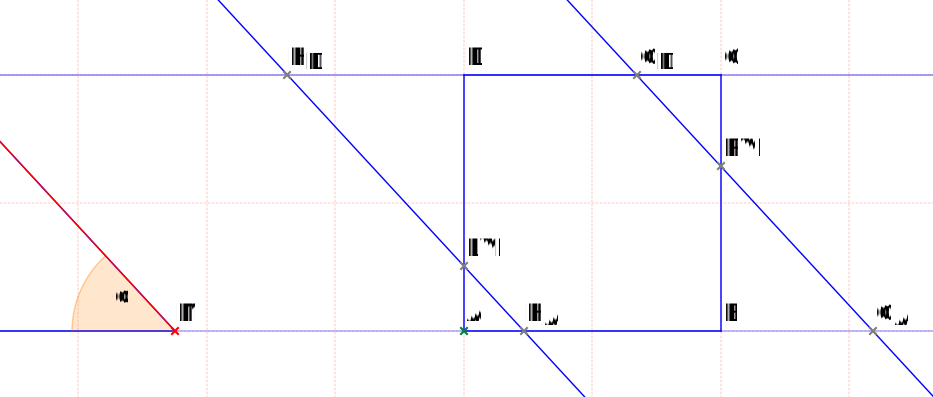
\includegraphics[width=\textwidth]{case2}
\begin{align*}
Effect &= 1 - (\frac{1}{2} * \overline{C\,RVI} * \overline{G_D\,C} + \frac{1}{2} * \overline{A\,LVI} * \overline{A\,H_A})\\
\overline{C\,RVI} &=  1 - \tan(\alpha) * \overline{B\,G_A}\\
\overline{A\,LVI} &=  1 - \tan(\alpha) * \overline{H_D\,D}
\end{align*}
\paragraph{Case 3:}
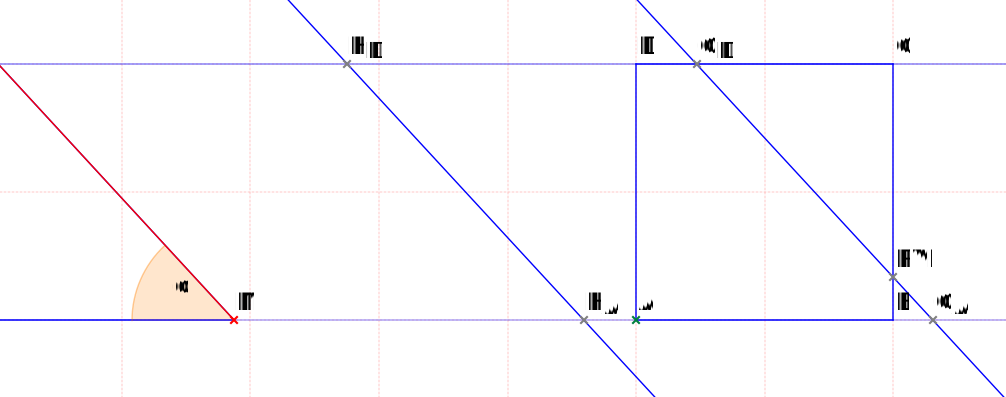
\includegraphics[width=\textwidth]{case3}

\end{document}